\documentclass[journal,12pt,twocolumn]{IEEEtran}
%
\usepackage{setspace}
\usepackage{gensymb}
%\doublespacing
\singlespacing

%\usepackage{graphicx}
%\usepackage{amssymb}
%\usepackage{relsize}
\usepackage[cmex10]{amsmath}
%\usepackage{amsthm}
%\interdisplaylinepenalty=2500
%\savesymbol{iint}
%\usepackage{txfonts}
%\restoresymbol{TXF}{iint}
%\usepackage{wasysym}
\usepackage{amsthm}
%\usepackage{iithtlc}
\usepackage{mathrsfs}
\usepackage{txfonts}
\usepackage{stfloats}
\usepackage{bm}
\usepackage{cite}
\usepackage{cases}
\usepackage{subfig}
%\usepackage{xtab}
\usepackage{longtable}
\usepackage{multirow}
%\usepackage{algorithm}
%\usepackage{algpseudocode}
\usepackage{enumitem}
\usepackage{mathtools}
\usepackage{tikz}
\usepackage[american]{circuitikz}
\usepackage{verbatim}
\usepackage{tfrupee}
\usepackage[breaklinks=true]{hyperref}
%\usepackage{stmaryrd}
\usepackage{tkz-euclide} % loads  TikZ and tkz-base
\usetkzobj{all}
\usetikzlibrary{decorations.markings}
\usetikzlibrary{shapes.geometric}
\newif\iflabrev
\usepackage{listings}
    \usepackage{color}                                            %%
    \usepackage{array}                                            %%
    \usepackage{longtable}                                        %%
    \usepackage{calc}                                             %%
    \usepackage{multirow}                                         %%
    \usepackage{hhline}                                           %%
    \usepackage{ifthen}                                           %%
  %optionally (for landscape tables embedded in another document): %%
    \usepackage{lscape}     
\usepackage{multicol}
\usepackage{chngcntr}
%\usepackage{enumerate}

%\usepackage{wasysym}
%\newcounter{MYtempeqncnt}
\DeclareMathOperator*{\Res}{Res}
%\renewcommand{\baselinestretch}{2}
\renewcommand\thesection{\arabic{section}}
\renewcommand\thesubsection{\thesection.\arabic{subsection}}
\renewcommand\thesubsubsection{\thesubsection.\arabic{subsubsection}}

\renewcommand\thesectiondis{\arabic{section}}
\renewcommand\thesubsectiondis{\thesectiondis.\arabic{subsection}}
\renewcommand\thesubsubsectiondis{\thesubsectiondis.\arabic{subsubsection}}

% correct bad hyphenation here
\hyphenation{op-tical net-works semi-conduc-tor}
\def\inputGnumericTable{}                                 %%

\lstset{
%language=C,
frame=single, 
breaklines=true,
columns=fullflexible
}
%\lstset{
%language=tex,
%frame=single, 
%breaklines=true
%}

\begin{document}
%


\newtheorem{theorem}{Theorem}[section]
\newtheorem{problem}{Problem}
\newtheorem{proposition}{Proposition}[section]
\newtheorem{lemma}{Lemma}[section]
\newtheorem{corollary}[theorem]{Corollary}
\newtheorem{example}{Example}[section]
\newtheorem{definition}[problem]{Definition}
%\newtheorem{thm}{Theorem}[section] 
%\newtheorem{defn}[thm]{Definition}
%\newtheorem{algorithm}{Algorithm}[section]
%\newtheorem{cor}{Corollary}
\newcommand{\BEQA}{\begin{eqnarray}}
\newcommand{\EEQA}{\end{eqnarray}}
\newcommand{\define}{\stackrel{\triangle}{=}}
\bibliographystyle{IEEEtran}
%\bibliographystyle{ieeetr}
\providecommand{\mbf}{\mathbf}
\providecommand{\pr}[1]{\ensuremath{\Pr\left(#1\right)}}
\providecommand{\qfunc}[1]{\ensuremath{Q\left(#1\right)}}
\providecommand{\sbrak}[1]{\ensuremath{{}\left[#1\right]}}
\providecommand{\lsbrak}[1]{\ensuremath{{}\left[#1\right.}}
\providecommand{\rsbrak}[1]{\ensuremath{{}\left.#1\right]}}
\providecommand{\brak}[1]{\ensuremath{\left(#1\right)}}
\providecommand{\lbrak}[1]{\ensuremath{\left(#1\right.}}
\providecommand{\rbrak}[1]{\ensuremath{\left.#1\right)}}
\providecommand{\cbrak}[1]{\ensuremath{\left\{#1\right\}}}
\providecommand{\lcbrak}[1]{\ensuremath{\left\{#1\right.}}
\providecommand{\rcbrak}[1]{\ensuremath{\left.#1\right\}}}
\theoremstyle{remark}
\newtheorem{rem}{Remark}
\newcommand{\sgn}{\mathop{\mathrm{sgn}}}
\providecommand{\abs}[1]{\left\vert#1\right\vert}
\providecommand{\res}[1]{\Res\displaylimits_{#1}} 
\providecommand{\norm}[1]{\left\lVert#1\right\rVert}
%\providecommand{\norm}[1]{\lVert#1\rVert}
\providecommand{\mtx}[1]{\mathbf{#1}}
\providecommand{\mean}[1]{E\left[ #1 \right]}
\providecommand{\fourier}{\overset{\mathcal{F}}{ \rightleftharpoons}}
%\providecommand{\hilbert}{\overset{\mathcal{H}}{ \rightleftharpoons}}
\providecommand{\system}{\overset{\mathcal{H}}{ \longleftrightarrow}}
	%\newcommand{\solution}[2]{\textbf{Solution:}{#1}}
\newcommand{\solution}{\noindent \textbf{Solution: }}
\newcommand{\cosec}{\,\text{cosec}\,}
\providecommand{\dec}[2]{\ensuremath{\overset{#1}{\underset{#2}{\gtrless}}}}
\newcommand{\myvec}[1]{\ensuremath{\begin{pmatrix}#1\end{pmatrix}}}
\newcommand{\mydet}[1]{\ensuremath{\begin{vmatrix}#1\end{vmatrix}}}
%\numberwithin{equation}{section}
\numberwithin{equation}{subsection}
%\numberwithin{problem}{section}
%\numberwithin{definition}{section}
\makeatletter
\@addtoreset{figure}{problem}
\makeatother
\let\StandardTheFigure\thefigure
\let\vec\mathbf
%\renewcommand{\thefigure}{\theproblem.\arabic{figure}}
\renewcommand{\thefigure}{\theproblem}
%\setlist[enumerate,1]{before=\renewcommand\theequation{\theenumi.\arabic{equation}}
%\counterwithin{equation}{enumi}
%\renewcommand{\theequation}{\arabic{subsection}.\arabic{equation}}
\def\putbox#1#2#3{\makebox[0in][l]{\makebox[#1][l]{}\raisebox{\baselineskip}[0in][0in]{\raisebox{#2}[0in][0in]{#3}}}}
     \def\rightbox#1{\makebox[0in][r]{#1}}
     \def\centbox#1{\makebox[0in]{#1}}
     \def\topbox#1{\raisebox{-\baselineskip}[0in][0in]{#1}}
     \def\midbox#1{\raisebox{-0.5\baselineskip}[0in][0in]{#1}}
\vspace{3cm}
\title{
%	\logo{
Wein-bridge oscillator
%	}
}
\author{ Vedala Sai Ashok$^{*}$% <-this % stops a space
	\thanks{*The author is with the Department
		of Electrical Engineering, Indian Institute of Technology, Hyderabad
		502285 India. All content in this manual is released under GNU GPL.  Free and open source.}
	
}	
%\title{
%	\logo{Matrix Analysis through Octave}{\begin{center}\includegraphics[scale=.24]{tlc}\end{center}}{}{HAMDSP}
%}
% paper title
% can use linebreaks \\ within to get better formatting as desired
%\title{Matrix Analysis through Octave}
%
%
% author names and IEEE memberships
% note positions of commas and nonbreaking spaces ( ~ ) LaTeX will not break
% a structure at a ~ so this keeps an author's name from being broken across
% two lines.
% use \thanks{} to gain access to the first footnote area
% a separate \thanks must be used for each paragraph as LaTeX2e's \thanks
% was not built to handle multiple paragraphs
%
%\author{<-this % stops a space
%\thanks{}}
%}
% note the % following the last \IEEEmembership and also \thanks - 
% these prevent an unwanted space from occurring between the last author name
% and the end of the author line. i.e., if you had this:
% 
% \author{....lastname \thanks{...} \thanks{...} }
%                     ^------------^------------^----Do not want these spaces!
%
% a space would be appended to the last name and could cause every name on that
% line to be shifted left slightly. This is one of those "LaTeX things". For
% instance, "\textbf{A} \textbf{B}" will typeset as "A B" not "AB". To get
% "AB" then you have to do: "\textbf{A}\textbf{B}"
% \thanks is no different in this regard, so shield the last } of each \thanks
% that ends a line with a % and do not let a space in before the next \thanks.
% Spaces after \IEEEmembership other than the last one are OK (and needed) as
% you are supposed to have spaces between the names. For what it is worth,
% this is a minor point as most people would not even notice if the said evil
% space somehow managed to creep in.
% The paper headers
%\markboth{Journal of \LaTeX\ Class Files,~Vol.~6, No.~1, January~2007}%
%{Shell \MakeLowercase{\textit{et al.}}: Bare Demo of IEEEtran.cls for Journals}
% The only time the second header will appear is for the odd numbered pages
% after the title page when using the twoside option.
% 
% *** Note that you probably will NOT want to include the author's ***
% *** name in the headers of peer review papers.                   ***
% You can use \ifCLASSOPTIONpeerreview for conditional compilation here if
% you desire.
% If you want to put a publisher's ID mark on the page you can do it like
% this:
%\IEEEpubid{0000--0000/00\$00.00~\copyright~2007 IEEE}
% Remember, if you use this you must call \IEEEpubidadjcol in the second
% column for its text to clear the IEEEpubid mark.
% make the title area
\maketitle
%\newpage
%\tableofcontents
\bigskip
\renewcommand{\thefigure}{\theenumi}
\renewcommand{\thetable}{\theenumi}
%\renewcommand{\theequation}{\theenumi}
%\begin{abstract}
%%\boldmath
%In this letter, an algorithm for evaluating the exact analytical bit error rate  (BER)  for the piecewise linear (PL) combiner for  multiple relays is presented. Previous results were available only for upto three relays. The algorithm is unique in the sense that  the actual mathematical expressions, that are prohibitively large, need not be explicitly obtained. The diversity gain due to multiple relays is shown through plots of the analytical BER, well supported by simulations. 
%
%\end{abstract}
% IEEEtran.cls defaults to using nonbold math in the Abstract.
% This preserves the distinction between vectors and scalars. However,
% if the journal you are submitting to favors bold math in the abstract,
% then you can use LaTeX's standard command \boldmath at the very start
% of the abstract to achieve this. Many IEEE journals frown on math
% in the abstract anyway.
% Note that keywords are not normally used for peerreview papers.
%\begin{IEEEkeywords}
%Cooperative diversity, decode and forward, piecewise linear
%\end{IEEEkeywords}
% For peer review papers, you can put extra information on the cover
% page as needed:
% \ifCLASSOPTIONpeerreview
% \begin{center} \bfseries EDICS Category: 3-BBND \end{center}
% \fi
%
% For peerreview papers, this IEEEtran command inserts a page break and
% creates the second title. It will be ignored for other modes.
%\IEEEpeerreviewmaketitle
%\begin{abstract}
%The objective of this manual is to introduce control system design at an elementary level.
%\end{abstract}
%\section{Feedback Circuits}
\begin{enumerate}[label=\arabic*.,ref=\theenumi]
%\begin{enumerate}[label=\thesubsection.\arabic*.,ref=\thesubsection.\theenumi]
\numberwithin{equation}{enumi}

\item  For the Wein-bridge oscillator of Fig \ref{fig:ee18btech11044_3_tikz_1}, use the expression for loop gain to find the poles of the closed-loop system. Give the expression for the pole, Q and use it to show that to locate the poles in the right half of s plane, $\frac{R_2}{R_1}$ must be selected to be greater than 2. 
\renewcommand{\thefigure}{\theenumi.\arabic{figure}}
\begin{figure}[!hbt]
	\begin{center}
			\resizebox{\columnwidth}{!}{\begin{circuitikz}
\ctikzset{bipoles/length=1cm}

\draw 
(0, 0) node[op amp] (opamp) {}
(opamp.-) -- (-1,0.35) -- (-1.5,0.35) to[R=$R_1$] (-3,0.35) -- (-3,0.33)node[ground]{}
(-1,0.35)-- (-1,1) to[R=$R_2$] (2,1) -- (2,0){}
(opamp.out)--(2,0){}
(opamp.+) -- (-1,-0.35) -- (-1,-1.5) to[C=$C$] (0.5,-1.5) to[R=$R$] (2,-1.5) -- (2,0){}
(-1,-1.5) -- (-1,-1.75)to[R=$R$] (-1,-2.5) -- (-1,-2.57)node[ground]{}
(0.5,-1.5) -- (0.5,-1.75) to[C=$C$] (0.5,-2.5) -- (0.5,-2.57)node[ground]{}
node at (2.3,0){$V_{out}$}



;\end{circuitikz}
}
	\end{center}
\caption{}
\label{fig:ee18btech11044_3_tikz_1}
\end{figure}



\item Compare the basic structure for a sinusoidal oscillator with Wein-bridge oscillator and give expressions for G and H. 

\solution
\begin{itemize}
 \item Comparring Fig \ref{fig:ee18btech11044_3_tikz_1} and Fig \ref{fig:ee18btech11044_3_tikz_2}, we get
\begin{align}
G = 1+\frac{R_2}{R_1} \label{eq:ee18btech11044_3_1}\\
H = \frac{Z_p}{Z_p + Z_s}  \label{eq:ee18btech11044_3_2}
\end{align}
where,
\begin{align}
    Z_p = \frac{R}{RSC+1} \\
    Z_s = \frac{RSC+1}{SC}
\end{align}
\end{itemize}



\begin{figure}[!hbt]
	\begin{center}
		\resizebox{\columnwidth}{!}{\tikzstyle{block} = [draw, fill=white!20, rectangle, 
    minimum height=3em, minimum width=6em]
\tikzstyle{sum} = [draw, fill=white!20, circle, node distance=1cm]
\tikzstyle{input} = [coordinate]
\tikzstyle{output} = [coordinate]
\tikzstyle{pinstyle} = [pin edge={to-,thin,black}]

\begin{tikzpicture}[auto, node distance=2cm,>=latex']
    \node [input, name=input] {};
    \node [sum, right of=input] (sum) {};
    \node [block, right of=sum] (controller) {$Amplifier$};
    \node [output, right of=controller] (output) {};
    \node [block, below of=controller] (feedback) {\tiny{Frequency selective network}};
    
    \draw [->] (sum) -- node {$V_i$} (controller);
    \draw [->] (controller) -- node [name=y] {$V_o$}(output);
    \draw [->] (y) |- (feedback);
    \draw [->] (feedback) -| node[pos=0.99]{$+$}  node [near end] {$V_f$} (sum);
\end{tikzpicture}
}
	\end{center}
\caption{}
\label{fig:ee18btech11044_3_tikz_2}
\end{figure} 


\item Write the closed loop Transfer function T(s) for wein-bridge oscillator.

\solution
\begin{align}
T(s) = \frac{(1+\frac{R_2}{R_1}) R^{2}C^{2}s^{2}+3RCs+1 }{R^{2}C^{2}s^{2}+(2-\frac{R_2}{R_1})RCs+1} \label{eq:ee18btech11044_3_7}
\end{align}





\item Write the characteristic equation for Wein-bridge oscillator.

\solution
\begin{align}
    1 - L(s) = 0  \\
    1 - \frac{1 + \frac{R_2}{R_1}}{3 + sCR + \frac{1}{sCR}} = 0  \\
    3 + sRC + \frac{1}{sCR} = 1 + \frac{R_2}{R_1}  \\
    3 - 1 +sRC +\frac{1}{sRC} -\frac{R_2}{R_1} = 0  \\
    2s + s^2 RC + \frac{1}{RC} -s\frac{R_2}{R_1} = 0  \\
    s^2 RC + s(2 - \frac{R_2}{R_1}) + \frac{1}{RC} =0 \\
    s^2 + s \frac{1}{RC}(2-\frac{R_2}{R_1}) + \frac{1}{R^2C^2} = 0 \label{eq:ee18btech11044_3_3}
\end{align}

\item
Write the general expression for the characteristic equation.

\solution
\begin{align}
    s^2 + s\frac{\omega_0}{Q} + \omega_0^2 = 0 \label{eq:ee18btech11044_3_4}
\end{align}

\item State the \textbf{Barkhausen criterion} for sustained oscillations with frequency $\omega_0$.

\solution
\begin{align}
    L(j\omega_0) = G(j\omega_0)  H(j\omega_0) = 1
\end{align}
\begin{itemize}
    \item That is, at $\omega_0$ the phase of the loop gain should be zero and the magnitude of loop gain should be 1.
    \item Only for a $\infty$ gain,system will produce a finite output for zero input. 
\end{itemize}

\item Give the definition of \textbf{Quality factor}(Q) and explain its significance.

\solution

\begin{itemize}
    \item It is a parameter of an oscillatory system expressing the relationship between stored energy and energy dissipation.
    \item The "purity" of output sine waves will be a function of the selectivity feedback network.
    \item That is, higher the value of Q for frequency selective network, the less the harmonic content of sine wave produced.
\end{itemize}
 


\item 
Compare the equations \ref{eq:ee18btech11044_3_3} and \ref{eq:ee18btech11044_3_4} and give expressions for Q and $\omega_0$

\solution
\begin{align}
    \omega_0^2 = \frac{1}{R^2C^2} \\
    \omega_0 = \frac{1}{RC} \label{eq:ee18btech11044_3_5} \\
    \frac{\omega_0}{Q} = \frac{1}{RC}(2 - \frac{R_2}{R_1}) \\
    Q = \frac{1}{(2 - \frac{R_2}{R_1})} \label{eq:ee18btech11044_3_6} \\
\end{align}
\item 
Using Eq \ref{eq:ee18btech11044_3_6} calculate the value of $\frac{R_2}{R_1}$ for which poles lie on right hand of s-plane.

\solution 

Poles lie on imaginary axis for $Q = \infty$
\begin{align}
    2 - \frac{R_2}{R_1} = 0 \\
    \frac{R_2}{R_1} = 2
\end{align}
$\therefore$ For poles to lie on right hand side of s-plane
\begin{align}
    \frac{R_2}{R_1} >2
\end{align}


\item
Verify the above theory using a Python code.

\solution

\begin{lstlisting}
codes/ee18btech11044/ee18btech11044_3_1.py
\end{lstlisting}
\begin{itemize}
    \item This figure shows how the location of poles vary if $\frac{R_2}{R_1}$ is varied for a fixed $\omega_0$.
    \item I have varied $\frac{R_2}{R_1}$ from -10 to 10. 
\end{itemize}

\begin{figure}[!ht]
\centering
\includegraphics[width=\columnwidth]{./figs/ee18btech11044/ee18btech11044_3_1.eps}
\caption{}
\label{fig:ee18btech11044_3_1}
\end{figure}

\item Choose appropriate values of Resistances and Capacitors to simulate the circuit.

\solution

\begin{table}[!ht]
\centering
%%%%%%%%%%%%%%%%%%%%%%%%%%%%%%%%%%%%%%%%%%%%%%%%%%%%%%%%%%%%%%%%%%%%%%
%%                                                                  %%
%%  This is the header of a LaTeX2e file exported from Gnumeric.    %%
%%                                                                  %%
%%  This file can be compiled as it stands or included in another   %%
%%  LaTeX document. The table is based on the longtable package so  %%
%%  the longtable options (headers, footers...) can be set in the   %%
%%  preamble section below (see PRAMBLE).                           %%
%%                                                                  %%
%%  To include the file in another, the following two lines must be %%
%%  in the including file:                                          %%
%%        \def\inputGnumericTable{}                                 %%
%%  at the beginning of the file and:                               %%
%%        \input{name-of-this-file.tex}                             %%
%%  where the table is to be placed. Note also that the including   %%
%%  file must use the following packages for the table to be        %%
%%  rendered correctly:                                             %%
%%    \usepackage[latin1]{inputenc}                                 %%
%%    \usepackage{color}                                            %%
%%    \usepackage{array}                                            %%
%%    \usepackage{longtable}                                        %%
%%    \usepackage{calc}                                             %%
%%    \usepackage{multirow}                                         %%
%%    \usepackage{hhline}                                           %%
%%    \usepackage{ifthen}                                           %%
%%  optionally (for landscape tables embedded in another document): %%
%%    \usepackage{lscape}                                           %%
%%                                                                  %%
%%%%%%%%%%%%%%%%%%%%%%%%%%%%%%%%%%%%%%%%%%%%%%%%%%%%%%%%%%%%%%%%%%%%%%



%%  This section checks if we are begin input into another file or  %%
%%  the file will be compiled alone. First use a macro taken from   %%
%%  the TeXbook ex 7.7 (suggestion of Han-Wen Nienhuys).            %%
\def\ifundefined#1{\expandafter\ifx\csname#1\endcsname\relax}


%%  Check for the \def token for inputed files. If it is not        %%
%%  defined, the file will be processed as a standalone and the     %%
%%  preamble will be used.                                          %%
\ifundefined{inputGnumericTable}

%%  We must be able to close or not the document at the end.        %%
	\def\gnumericTableEnd{\end{document}}


%%%%%%%%%%%%%%%%%%%%%%%%%%%%%%%%%%%%%%%%%%%%%%%%%%%%%%%%%%%%%%%%%%%%%%
%%                                                                  %%
%%  This is the PREAMBLE. Change these values to get the right      %%
%%  paper size and other niceties.                                  %%
%%                                                                  %%
%%%%%%%%%%%%%%%%%%%%%%%%%%%%%%%%%%%%%%%%%%%%%%%%%%%%%%%%%%%%%%%%%%%%%%

	\documentclass[12pt%
			  %,landscape%
                    ]{report}
       \usepackage[latin1]{inputenc}
       \usepackage{fullpage}
       \usepackage{color}
       \usepackage{array}
       \usepackage{longtable}
       \usepackage{calc}
       \usepackage{multirow}
       \usepackage{hhline}
       \usepackage{ifthen}

	\begin{document}


%%  End of the preamble for the standalone. The next section is for %%
%%  documents which are included into other LaTeX2e files.          %%
\else

%%  We are not a stand alone document. For a regular table, we will %%
%%  have no preamble and only define the closing to mean nothing.   %%
    \def\gnumericTableEnd{}

%%  If we want landscape mode in an embedded document, comment out  %%
%%  the line above and uncomment the two below. The table will      %%
%%  begin on a new page and run in landscape mode.                  %%
%       \def\gnumericTableEnd{\end{landscape}}
%       \begin{landscape}


%%  End of the else clause for this file being \input.              %%
\fi

%%%%%%%%%%%%%%%%%%%%%%%%%%%%%%%%%%%%%%%%%%%%%%%%%%%%%%%%%%%%%%%%%%%%%%
%%                                                                  %%
%%  The rest is the gnumeric table, except for the closing          %%
%%  statement. Changes below will alter the table's appearance.     %%
%%                                                                  %%
%%%%%%%%%%%%%%%%%%%%%%%%%%%%%%%%%%%%%%%%%%%%%%%%%%%%%%%%%%%%%%%%%%%%%%

\providecommand{\gnumericmathit}[1]{#1} 
%%  Uncomment the next line if you would like your numbers to be in %%
%%  italics if they are italizised in the gnumeric table.           %%
%\renewcommand{\gnumericmathit}[1]{\mathit{#1}}
\providecommand{\gnumericPB}[1]%
{\let\gnumericTemp=\\#1\let\\=\gnumericTemp\hspace{0pt}}
 \ifundefined{gnumericTableWidthDefined}
        \newlength{\gnumericTableWidth}
        \newlength{\gnumericTableWidthComplete}
        \newlength{\gnumericMultiRowLength}
        \global\def\gnumericTableWidthDefined{}
 \fi
%% The following setting protects this code from babel shorthands.  %%
 \ifthenelse{\isundefined{\languageshorthands}}{}{\languageshorthands{english}}
%%  The default table format retains the relative column widths of  %%
%%  gnumeric. They can easily be changed to c, r or l. In that case %%
%%  you may want to comment out the next line and uncomment the one %%
%%  thereafter                                                      %%
\providecommand\gnumbox{\makebox[0pt]}
%%\providecommand\gnumbox[1][]{\makebox}

%% to adjust positions in multirow situations                       %%
\setlength{\bigstrutjot}{\jot}
\setlength{\extrarowheight}{\doublerulesep}

%%  The \setlongtables command keeps column widths the same across  %%
%%  pages. Simply comment out next line for varying column widths.  %%
\setlongtables

\setlength\gnumericTableWidth{%
	53pt+%
	93pt+%
0pt}
\def\gumericNumCols{2}
\setlength\gnumericTableWidthComplete{\gnumericTableWidth+%
         \tabcolsep*\gumericNumCols*2+\arrayrulewidth*\gumericNumCols}
\ifthenelse{\lengthtest{\gnumericTableWidthComplete > \linewidth}}%
         {\def\gnumericScale{\ratio{\linewidth-%
                        \tabcolsep*\gumericNumCols*2-%
                        \arrayrulewidth*\gumericNumCols}%
{\gnumericTableWidth}}}%
{\def\gnumericScale{1}}

%%%%%%%%%%%%%%%%%%%%%%%%%%%%%%%%%%%%%%%%%%%%%%%%%%%%%%%%%%%%%%%%%%%%%%
%%                                                                  %%
%% The following are the widths of the various columns. We are      %%
%% defining them here because then they are easier to change.       %%
%% Depending on the cell formats we may use them more than once.    %%
%%                                                                  %%
%%%%%%%%%%%%%%%%%%%%%%%%%%%%%%%%%%%%%%%%%%%%%%%%%%%%%%%%%%%%%%%%%%%%%%

\ifthenelse{\isundefined{\gnumericColA}}{\newlength{\gnumericColA}}{}\settowidth{\gnumericColA}{\begin{tabular}{@{}p{53pt*\gnumericScale}@{}}x\end{tabular}}
\ifthenelse{\isundefined{\gnumericColB}}{\newlength{\gnumericColB}}{}\settowidth{\gnumericColB}{\begin{tabular}{@{}p{93pt*\gnumericScale}@{}}x\end{tabular}}

\begin{tabular}[c]{%
	b{\gnumericColA}%
	b{\gnumericColB}%
	}

%%%%%%%%%%%%%%%%%%%%%%%%%%%%%%%%%%%%%%%%%%%%%%%%%%%%%%%%%%%%%%%%%%%%%%
%%  The longtable options. (Caption, headers... see Goosens, p.124) %%
%	\caption{The Table Caption.}             \\	%
% \hline	% Across the top of the table.
%%  The rest of these options are table rows which are placed on    %%
%%  the first, last or every page. Use \multicolumn if you want.    %%

%%  Header for the first page.                                      %%
%	\multicolumn{2}{c}{The First Header} \\ \hline 
%	\multicolumn{1}{c}{colTag}	%Column 1
%	&\multicolumn{1}{c}{colTag}	\\ \hline %Last column
%	\endfirsthead

%%  The running header definition.                                  %%
%	\hline
%	\multicolumn{2}{l}{\ldots\small\slshape continued} \\ \hline
%	\multicolumn{1}{c}{colTag}	%Column 1
%	&\multicolumn{1}{c}{colTag}	\\ \hline %Last column
%	\endhead

%%  The running footer definition.                                  %%
%	\hline
%	\multicolumn{2}{r}{\small\slshape continued\ldots} \\
%	\endfoot

%%  The ending footer definition.                                   %%
%	\multicolumn{2}{c}{That's all folks} \\ \hline 
%	\endlastfoot
%%%%%%%%%%%%%%%%%%%%%%%%%%%%%%%%%%%%%%%%%%%%%%%%%%%%%%%%%%%%%%%%%%%%%%

\hhline{|-|-}
	 \multicolumn{1}{|p{\gnumericColA}|}%
	{\gnumericPB{\centering}\gnumbox{\textbf{Parameter}}}
	&\multicolumn{1}{p{\gnumericColB}|}%
	{\gnumericPB{\centering}\gnumbox{\textbf{Value}}}
\\
\hhline{|--|}
	 \multicolumn{1}{|p{\gnumericColA}|}%
	{\gnumericPB{\raggedright}\gnumbox[l]{$R_{1}$}}
	&\multicolumn{1}{p{\gnumericColB}|}%
	{\gnumericPB{\raggedright}\gnumbox[l]{$10k\Omega$}}
\\
\hhline{|--|}
	 \multicolumn{1}{|p{\gnumericColA}|}%
	{\gnumericPB{\raggedright}\gnumbox[l]{$R_{2}$}}
	&\multicolumn{1}{p{\gnumericColB}|}%
	{\gnumericPB{\raggedright}\gnumbox[l]{$20.3k\Omega$}}
\\
\hhline{|--|}
	 \multicolumn{1}{|p{\gnumericColA}|}%
	{\gnumericPB{\raggedright}\gnumbox[l]{$R_{p}$}}
	&\multicolumn{1}{p{\gnumericColB}|}%
	{\gnumericPB{\raggedright}\gnumbox[l]{$10k\Omega$}}
\\
\hhline{|--|}
	 \multicolumn{1}{|p{\gnumericColA}|}%
	{\gnumericPB{\raggedright}\gnumbox[l]{$R_{s}$}}
	&\multicolumn{1}{p{\gnumericColB}|}%
	{\gnumericPB{\raggedright}\gnumbox[l]{$10k\Omega$}}
\\
\hhline{|--|}
	 \multicolumn{1}{|p{\gnumericColA}|}%
	{\gnumericPB{\raggedright}\gnumbox[l]{$C_{s}$}}
	&\multicolumn{1}{p{\gnumericColB}|}%
	{\gnumericPB{\raggedright}\gnumbox[l]{$16nF$}}
\\
\hhline{|--|}
	 \multicolumn{1}{|p{\gnumericColA}|}%
	{\gnumericPB{\raggedright}\gnumbox[l]{$R_{p}$}}
	&\multicolumn{1}{p{\gnumericColB}|}%
	{\gnumericPB{\raggedright}\gnumbox[l]{$10k\Omega$}}
\\
\hhline{|--|}
	 \multicolumn{1}{|p{\gnumericColA}|}%
	{\gnumericPB{\raggedright}\gnumbox[l]{$C_{p}$}}
	&\multicolumn{1}{p{\gnumericColB}|}%
	{\gnumericPB{\raggedright}\gnumbox[l]{$16nF$}}

\\
\hhline{|-|-|}
\end{tabular}

\ifthenelse{\isundefined{\languageshorthands}}{}{\languageshorthands{\languagename}}
\gnumericTableEnd

\caption{}
\label{table:ee18btech11044_t_1}
\end{table}

Where, according to Fig \ref{fig:ee18btech11044_3_tikz_1}
\begin{align}
    R_p = R_s = R \\
    C_p = C_s = C
\end{align}

%Case-------------------------1

\item Calculate the frequency of sinusoid generated for the values given in table \ref{table:ee18btech11044_t_1}.

\solution

\begin{itemize}
\item Calculating poles of transfer function for $\frac{R_2}{R_1}$= 2.03 using a python script.
\begin{lstlisting}
codes/ee18btech11044/ee18btech11044_3_1.py
\end{lstlisting}
\item We get the poles as 93.75 + j 6249.2968 and 93.75 - j 6249.2968, which correspond to an exponentially increasing sinusoid of  frequency  995.11Hz. 
\end{itemize}

%%%%%%%%%%%%%%%%%%%%%%%%%%Python simulation

\item Substituting the values shown in table \ref{table:ee18btech11044_t_1} in the Eq \ref{eq:ee18btech11044_3_7}, Plot the impulse response and step response using a python code.

\solution

\begin{itemize}
\item Refer Fig \ref{fig:ee18btech11044_3_2} for impulse response of transfer function.
\item Code for generating impulse response
\begin{lstlisting}
codes/ee18btech11044/ee18btech11044_3_2.py
\end{lstlisting}
\item Refer D=Fig \ref{fig:ee18btech11044_3_3} for step response of transfer function.
\item Code for generating step response
\begin{lstlisting}
codes/ee18btech11044/ee18btech11044_3_3.py
\end{lstlisting}
\item As expected from the poles we are getting an exponentially increasing sinusoid as both impulse response and step response.
\end{itemize}

\begin{figure}[!ht]
\centering
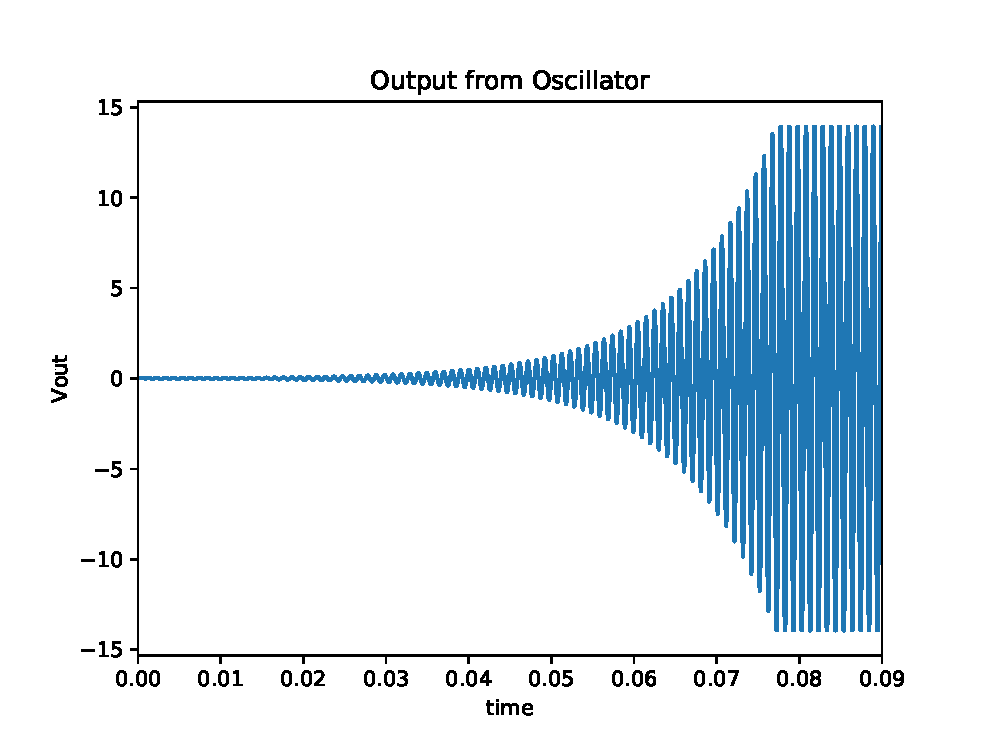
\includegraphics[width=\columnwidth]{./figs/ee18btech11044/ee18btech11044_3_2.eps}
\caption{}
\label{fig:ee18btech11044_3_2}
\end{figure}

\begin{figure}[!ht]
\centering
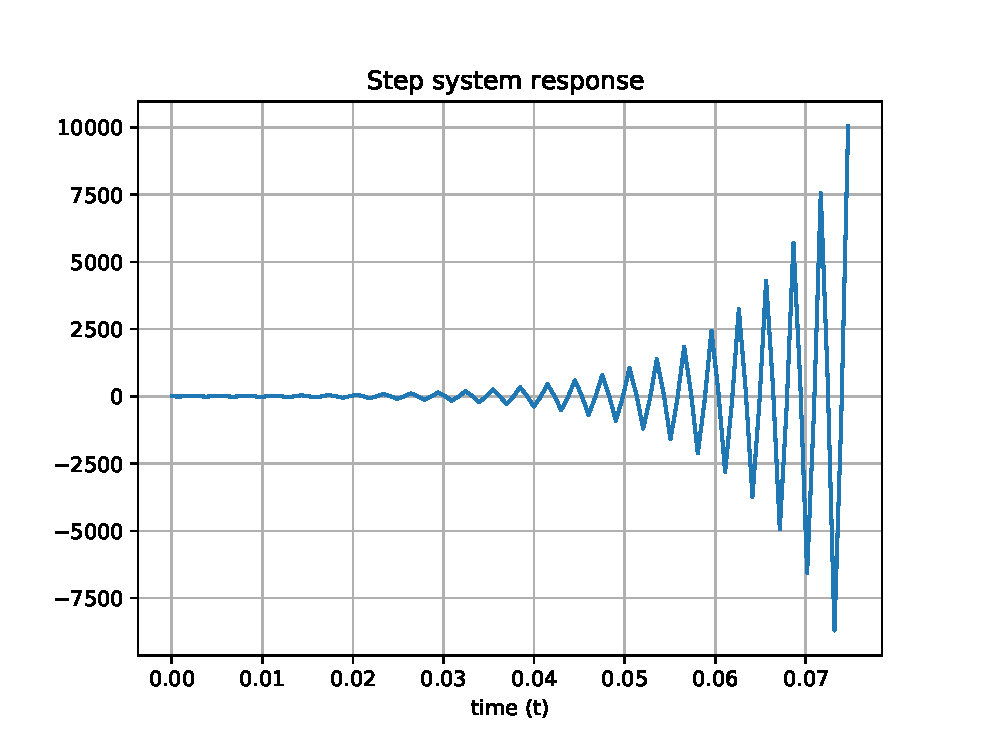
\includegraphics[width=\columnwidth]{./figs/ee18btech11044/ee18btech11044_3_3.eps}
\caption{}
\label{fig:ee18btech11044_3_3}
\end{figure}

%%%%%%%%%%%%%%%%%%%%%%%%Spice simulation

\item Simulate the circuit shown in Fig \ref{fig:ee18btech11044_3_tikz_1} using spice simulators. Substitute the values shown in table \ref{table:ee18btech11044_t_1} and plot the output using a python script.

\solution

\begin{itemize}
\item Refer Fig \ref{fig:ee18btech11044_3_4} for the spice simulation output.  
\item You can find the netlist for the simulated circuit here:
\begin{lstlisting}
spice/ee18btech11044/ee18btech11044_3_1.net
\end{lstlisting}
\item You can find the python script used to generate the output here:
\begin{lstlisting}
spice/ee18btech11044/ee18btech11044_spice_3_1.py
\end{lstlisting}
\end{itemize}

\begin{figure}[!ht]
\centering
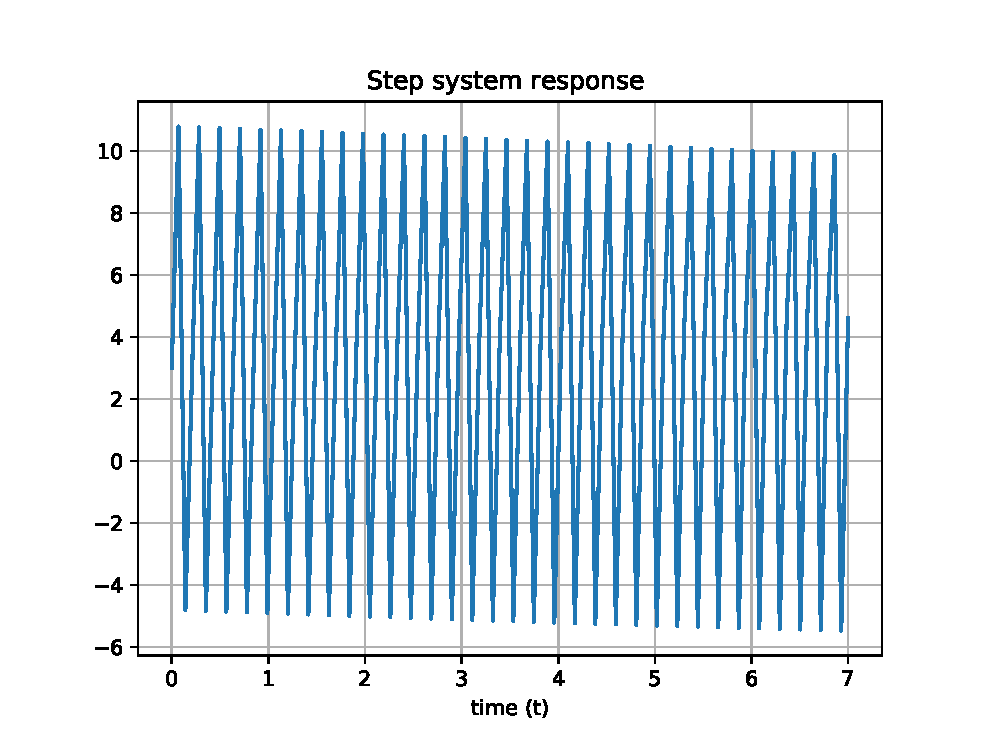
\includegraphics[width=\columnwidth]{./figs/ee18btech11044/ee18btech11044_3_4.eps}
\label{fig:ee18btech11044_3_4}
\caption{}
\end{figure}

%%%%%%%%%%%%%%%%%%%%%%%Frequency of spice simulation

\item Calculate the frequency of sinusoidal wave using plot generated from simulation.
 
 \solution
 \begin{itemize}
     \item Consider a part of plot generated from simulation shown in the Fig \ref{fig:ee18btech11044_3_5}.
     \item Calculating the Time-period of the sinusoidal wave generated using the two points marked in the Fig \ref{fig:ee18btech11044_3_5}.
     \begin{align}
         T_0 = 0.0856452 - 0.0846361 \\
         f_0 = 1/T_0 \\
         f_0 = 990.98Hz.
     \end{align}
     \item We get the frequencies calculated from the formulae and the plot to be approximately same.
     \item Use this script to generate Fig \ref{fig:ee18btech11044_3_5}
\begin{lstlisting}
spice/ee18btech11044/ee18btech11044_spice_3_2.py
\end{lstlisting}
 \end{itemize}
 

 
\begin{figure}[!ht]
\centering
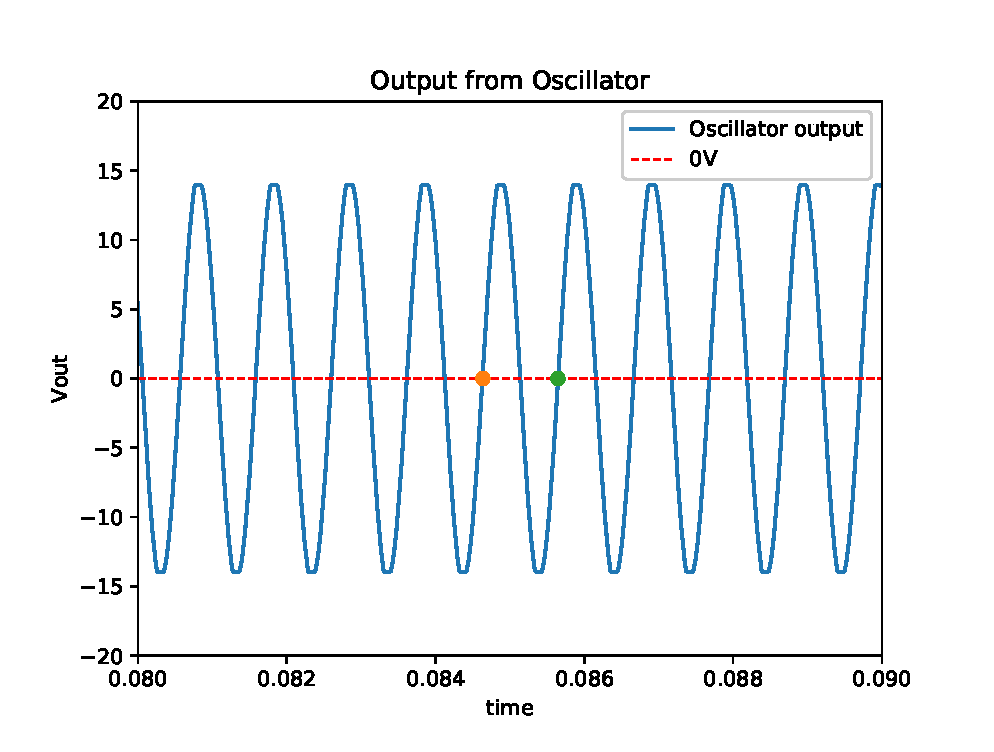
\includegraphics[width=\columnwidth]{./figs/ee18btech11044/ee18btech11044_3_5.eps}
\caption{}
\label{fig:ee18btech11044_3_5}
\end{figure}

%Case------------------------------------------------2
\item Calculate the poles of transfer function when the ratio $\frac{R_2}{R_1}$ is taken to be 2.

\solution

\begin{itemize}
\item Calculating poles of transfer function for $\frac{R_2}{R_1}$= 2 using a python script.
\begin{lstlisting}
codes/ee18btech11044/ee18btech11044_3_4.py
\end{lstlisting}
\item We get the poles to be purely imaginery +6250j and -6250j, which correspond to a sinusoid of frequency  995.22Hz. 
\end{itemize}

%%%%%%%%%%%%%%%%%%%%%%python simulation
\item Substituting the values shown in table \ref{table:ee18btech11044_t_1} in the Eq \ref{eq:ee18btech11044_3_7}, Consider the ratio of $\frac{R_2}{R_1}$ = 2 and plot the impulse response and step response using a python code.

\solution

\begin{itemize}
\item Refer Fig \ref{fig:ee18btech11044_3_6} for impulse response of transfer function.
\item Code for generating impulse response
\begin{lstlisting}
codes/ee18btech11044/ee18btech11044_3_5.py
\end{lstlisting}
\item Refer D=Fig \ref{fig:ee18btech11044_3_7} for step response of transfer function.
\item Code for generating step response
\begin{lstlisting}
codes/ee18btech11044/ee18btech11044_3_6.py
\end{lstlisting}
\item As expected from the poles we are getting pure sinusoid as both impulse response and step response.
\end{itemize}

\begin{figure}[!ht]
\centering
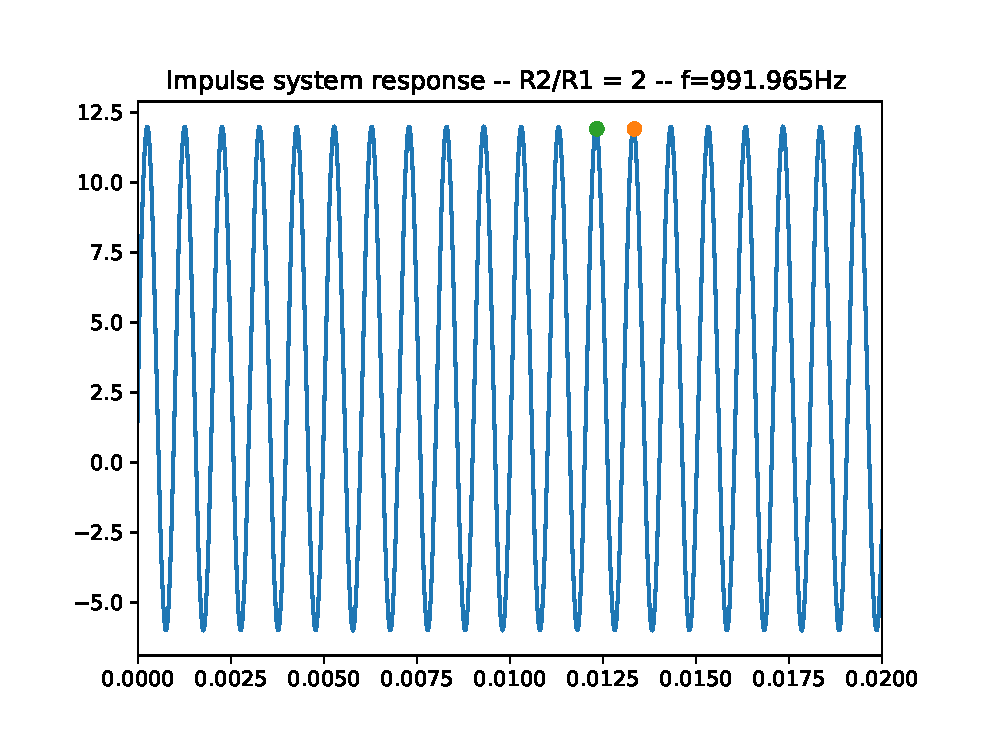
\includegraphics[width=\columnwidth]{./figs/ee18btech11044/ee18btech11044_3_6.eps}
\caption{}
\label{fig:ee18btech11044_3_6}
\end{figure}

\begin{figure}[!ht]
\centering
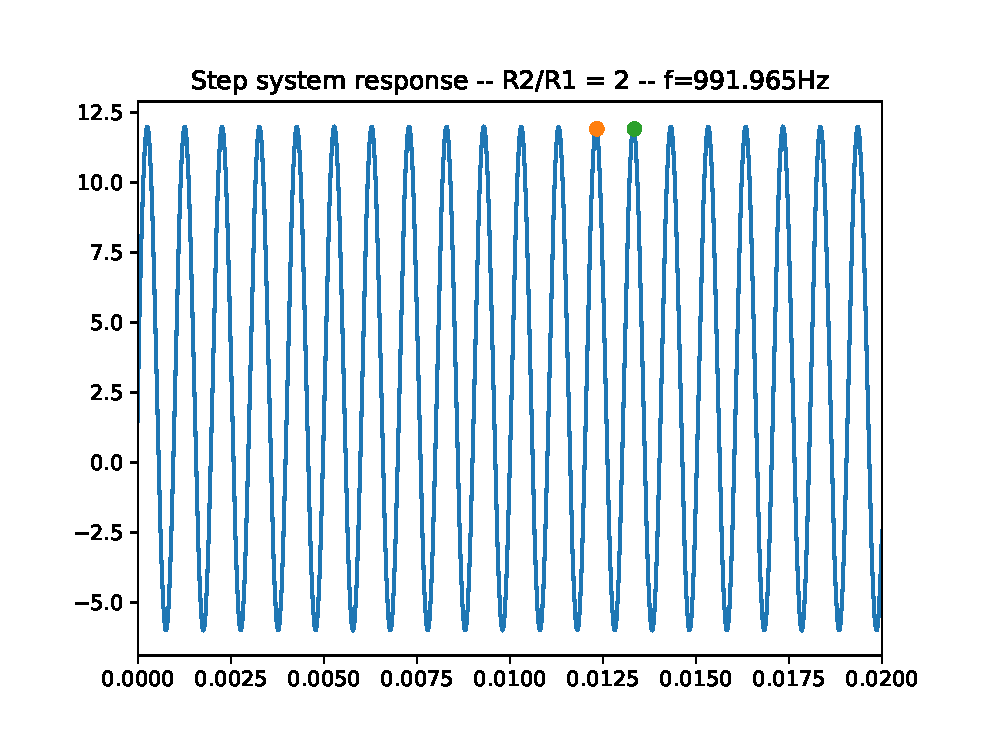
\includegraphics[width=\columnwidth]{./figs/ee18btech11044/ee18btech11044_3_7.eps}
\caption{}
\label{fig:ee18btech11044_3_7}
\end{figure}

%%%%%%%%%%%%%%%%%%%%%%%%%%%%%%spice simulation
\begin{figure}[!ht]
\centering
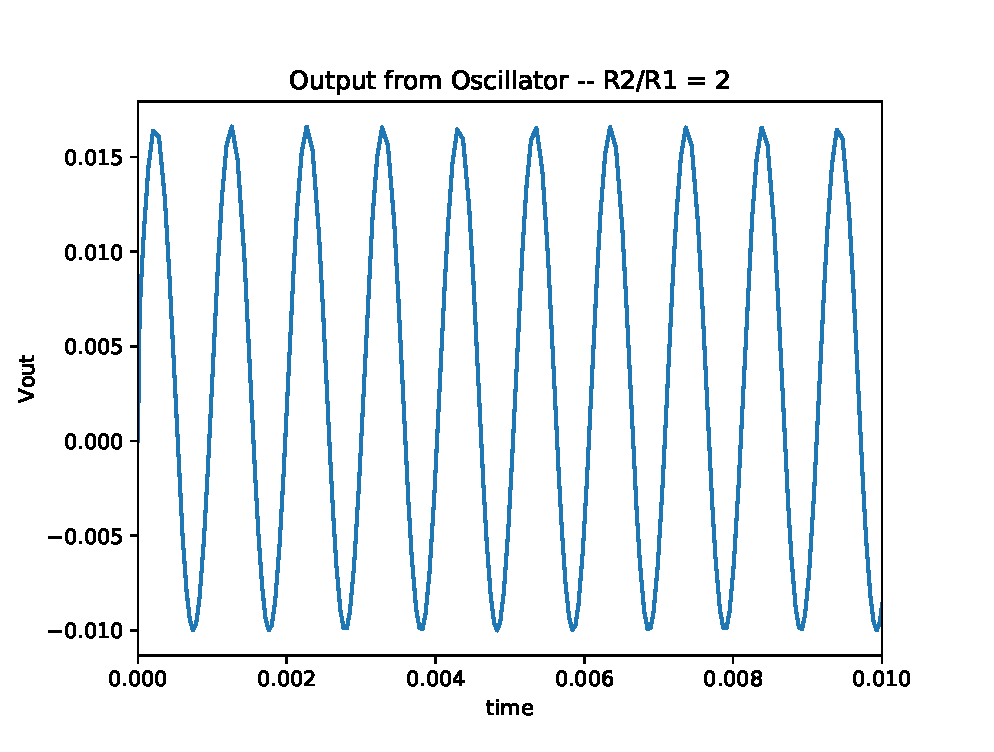
\includegraphics[width=\columnwidth]{./figs/ee18btech11044/ee18btech11044_3_8.eps}
\label{fig:ee18btech11044_3_8}
\caption{}
\end{figure}

\item Simulate the circuit shown in Fig \ref{fig:ee18btech11044_3_tikz_1} using spice simulators. Consider the ratio of $\frac{R_2}{R_1}$ = 2 and plot the output using a python script.

\solution

\begin{itemize}
\item Refer Fig \ref{fig:ee18btech11044_3_8} for the spice simulation output.  
\item You can find the netlist for the simulated circuit here:
\begin{lstlisting}
spice/ee18btech11044/ee18btech11044_3_2.net
\end{lstlisting}
\item You can find the python script used to generate the output here:
\begin{lstlisting}
spice/ee18btech11044/ee18btech11044_spice_3_3.py
\end{lstlisting}
\end{itemize}



%%%%%%%%%%%%%%%%%%%%%%%Frequency of spice simulation

\item Calculate the frequency of sinusoidal wave using plot generated from simulationfor the case where $\frac{R_2}{R_1} =2$.
 
 \solution
 \begin{itemize}
     \item Consider a part of plot generated from simulation shown in the Fig \ref{fig:ee18btech11044_3_9}.
     \item Calculating the Time-period of the sinusoidal wave generated using the two points marked in the Fig \ref{fig:ee18btech11044_3_9}.
     \begin{align}
         T_0 = 0.00227823 - 0.00127016 \\
         f_0 = 1/T_0 \\
         f_0 = 991.9944Hz.
     \end{align}
     \item We get the frequencies calculated from the formulae and the plot to be approximately same.
     \item Use this script to generate Fig \ref{fig:ee18btech11044_3_9}
\begin{lstlisting}
spice/ee18btech11044/ee18btech11044_spice_3_4.py
\end{lstlisting}
 \end{itemize}
 

 
\begin{figure}[!ht]
\centering
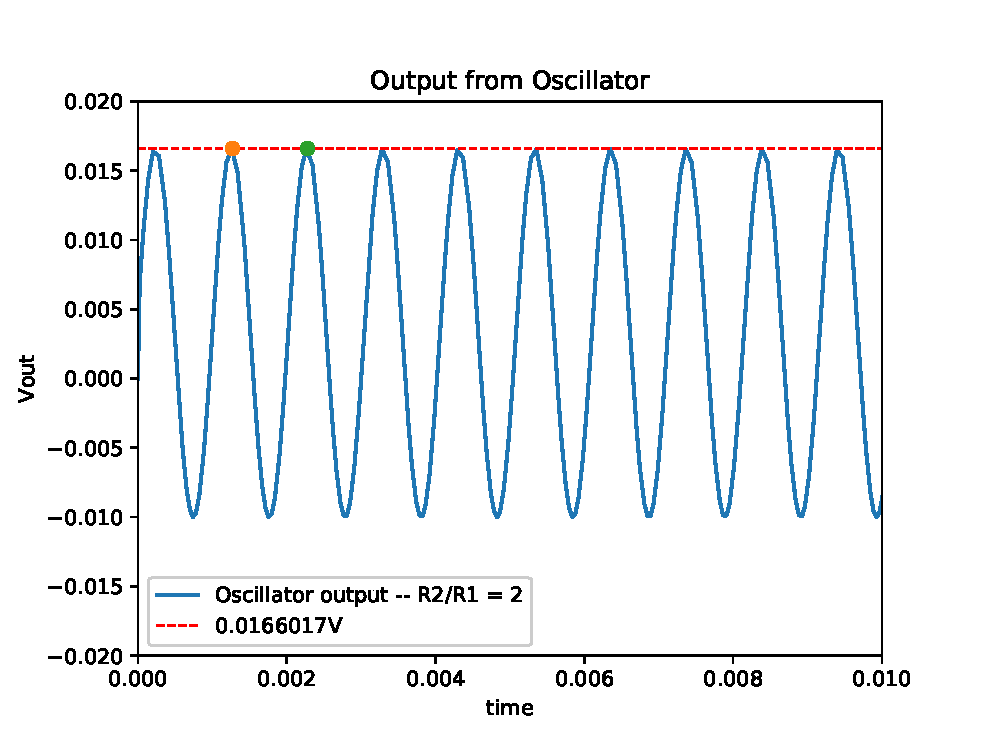
\includegraphics[width=\columnwidth]{./figs/ee18btech11044/ee18btech11044_3_9.eps}
\caption{}
\label{fig:ee18btech11044_3_9}
\end{figure}



%%%%%%%%%%%%%%%%%%%%%%%%%%%Case--------------3
\item Calculate the poles of transfer function when the ratio $\frac{R_2}{R_1}$ is taken to be 9.

\solution

\begin{itemize}
\item Calculating poles of transfer function for $\frac{R_2}{R_1}$= 9 using a python script.
\begin{lstlisting}
codes/ee18btech11044/ee18btech11044_3_7.py
\end{lstlisting}
\item We get the poles two real and distinct poles at 42838.13728906053  and  911.8627109394729, which correspond to an exponentially increasing function.  
\end{itemize}

%%%%%%%%%%%%%%%%%%%%%%python simulation
\item Substituting the values shown in table \ref{table:ee18btech11044_t_1} in the Eq \ref{eq:ee18btech11044_3_7}. Consider the ratio of $\frac{R_2}{R_1}$ = 9 and plot the impulse response and step response using a python code.

\solution

\begin{itemize}
\item Refer Fig \ref{fig:ee18btech11044_3_10} for impulse response of transfer function.
\item Code for generating impulse response
\begin{lstlisting}
codes/ee18btech11044/ee18btech11044_3_8.py
\end{lstlisting}
\item Refer Fig \ref{fig:ee18btech11044_3_11} for step response of transfer function.
\item Code for generating step response
\begin{lstlisting}
codes/ee18btech11044/ee18btech11044_3_9.py
\end{lstlisting}
\item As expected from the poles we are getting an exponentially increasing function as both impulse response and step response.
\end{itemize}

\begin{figure}[!ht]
\centering
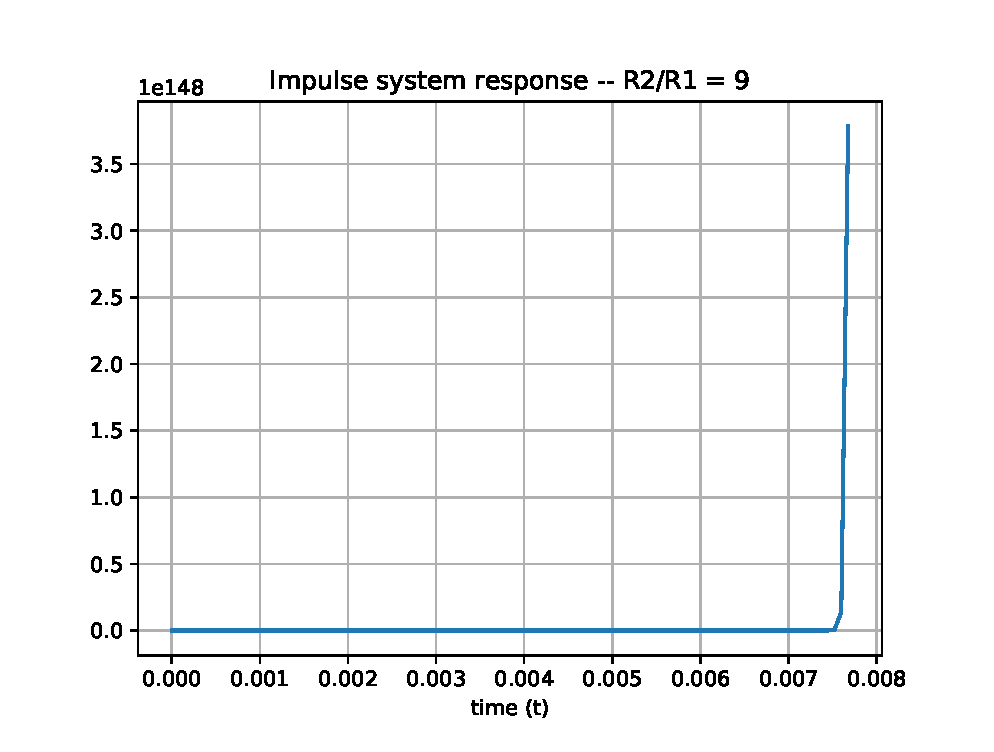
\includegraphics[width=\columnwidth]{./figs/ee18btech11044/ee18btech11044_3_10.eps}
\caption{}
\label{fig:ee18btech11044_3_10}
\end{figure}

\begin{figure}[!ht]
\centering
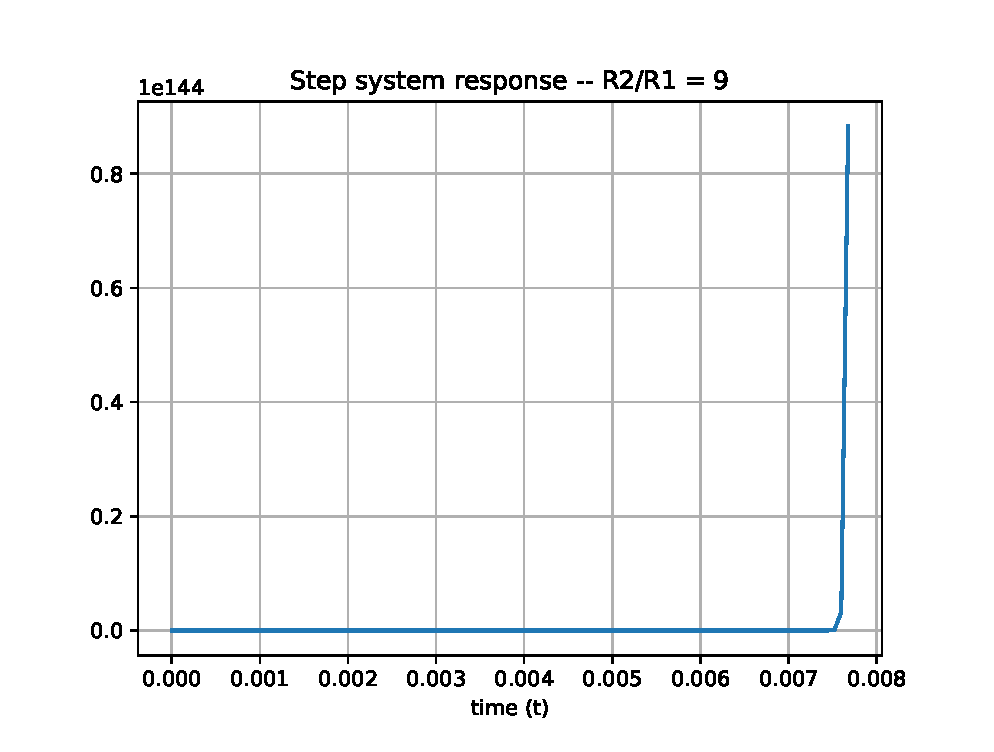
\includegraphics[width=\columnwidth]{./figs/ee18btech11044/ee18btech11044_3_11.eps}
\caption{}
\label{fig:ee18btech11044_3_11}
\end{figure}

%%%%%%%%%%%%%%%%%%%%%%%%%%%%%%spice simulation
\item Simulate the circuit shown in Fig \ref{fig:ee18btech11044_3_tikz_1} using spice simulators. Consider the ratio of $\frac{R_2}{R_1}$ = 9 and plot the output using a python script.

\solution

\begin{itemize}
\item Refer Fig \ref{fig:ee18btech11044_3_12} for the spice simulation output.  
\item You can find the netlist for the simulated circuit here:
\begin{lstlisting}
spice/ee18btech11044/ee18btech11044_3_3.net
\end{lstlisting}
\item You can find the python script used to generate the output here:
\begin{lstlisting}
spice/ee18btech11044/ee18btech11044_spice_3_5.py
\end{lstlisting}
\end{itemize}

\begin{figure}[!ht]
\centering
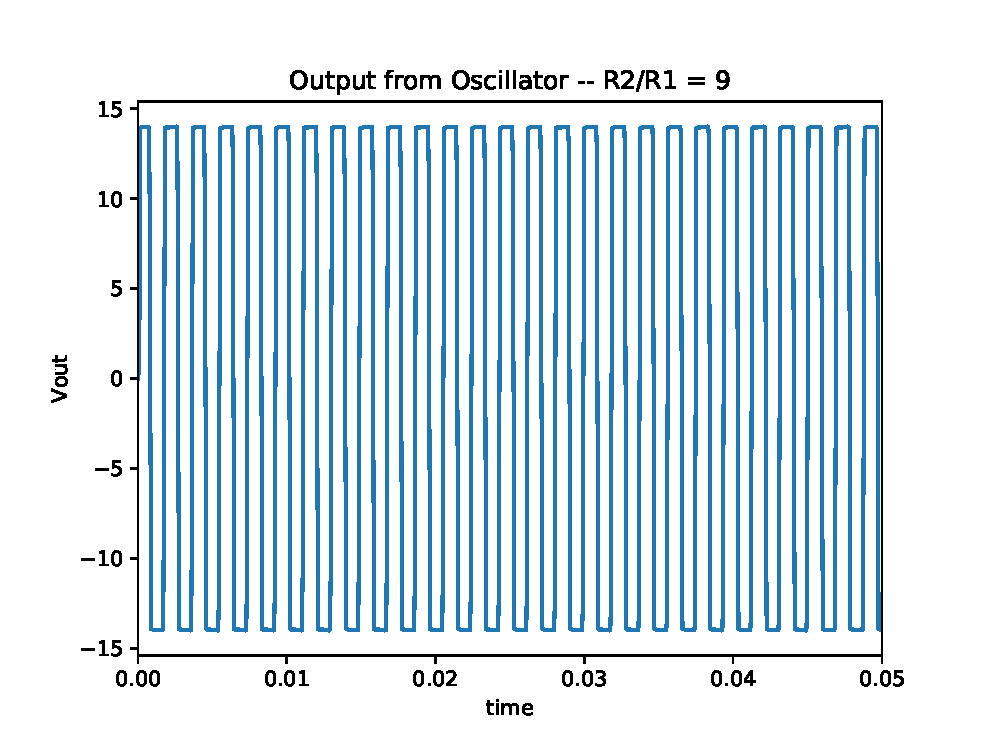
\includegraphics[width=\columnwidth]{./figs/ee18btech11044/ee18btech11044_3_12.eps}
\label{fig:ee18btech11044_3_12}
\caption{}
\end{figure}

%%%%%%%%%%%%%%%%%%%%%%%Frequency of spice simulation

\item Calculate the frequency of sinusoidal wave using plot generated from simulationfor the case where $\frac{R_2}{R_1} = 9$.
 
 \solution
 \begin{itemize}
     \item Consider a part of plot generated from simulation shown in the Fig \ref{fig:ee18btech11044_3_13}.
     \item Calculating the Time-period of the sinusoidal wave generated using the two points marked in the Fig \ref{fig:ee18btech11044_3_13}.
     \begin{align}
         T_0 = 0.00453629 - 0.00270161 \\
         f_0 = 1/T_0 \\
         f_0 = 545.054Hz.
     \end{align}
     \item Use this script to generate Fig \ref{fig:ee18btech11044_3_13}
\begin{lstlisting}
spice/ee18btech11044/ee18btech11044_spice_3_6.py
\end{lstlisting}
\item In this case because of the saturation voltage in op-amp we are getting a curve similar to square wave.
 \end{itemize}
 

 
\begin{figure}[!ht]
\centering
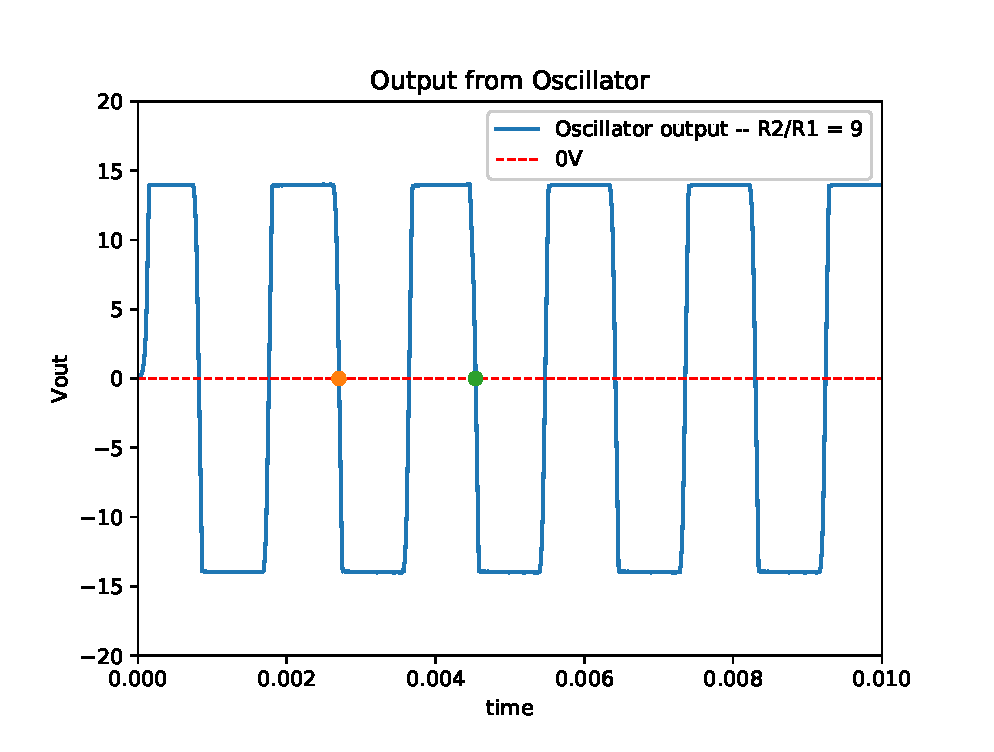
\includegraphics[width=\columnwidth]{./figs/ee18btech11044/ee18btech11044_3_13.eps}
\caption{}
\label{fig:ee18btech11044_3_13}
\end{figure}

%%%%%%%%%%%%%%%%%%%%%%%%%%%Case--------------4
\item Calculate the poles of transfer function when the ratio $\frac{R_2}{R_1}$ is taken to be 1.5.

\solution

\begin{itemize}
\item Calculating poles of transfer function for $\frac{R_2}{R_1}$= 1.5 using a python script.
\begin{lstlisting}
codes/ee18btech11044/ee18btech11044_3_10.py
\end{lstlisting}
\item We get the poles two complex conjugate poles in Left Hand Side of s-plane at  -1563+6051.5364784490885j and -1563-6051.5364784490885j, which correspond to an exponentially decreasing sinusoid function, corresponding to a frequnecy of 963.27Hz. 
\end{itemize}

%%%%%%%%%%%%%%%%%%%%%%python simulation
\item Substituting the values shown in table \ref{table:ee18btech11044_t_1} in the Eq \ref{eq:ee18btech11044_3_7}. Consider the ratio of $\frac{R_2}{R_1}$ = 1.5 and plot the impulse response and step response using a python code.

\solution

\begin{itemize}
\item Refer Fig \ref{fig:ee18btech11044_3_14} for impulse response of transfer function.
\item Code for generating impulse response
\begin{lstlisting}
codes/ee18btech11044/ee18btech11044_3_11.py
\end{lstlisting}
\item Refer Fig \ref{fig:ee18btech11044_3_15} for step response of transfer function.
\item Code for generating step response
\begin{lstlisting}
codes/ee18btech11044/ee18btech11044_3_12.py
\end{lstlisting}
\item As expected from the poles we are getting an exponentially increasing function as both impulse response and step response.
\end{itemize}

\begin{figure}[!ht]
\centering
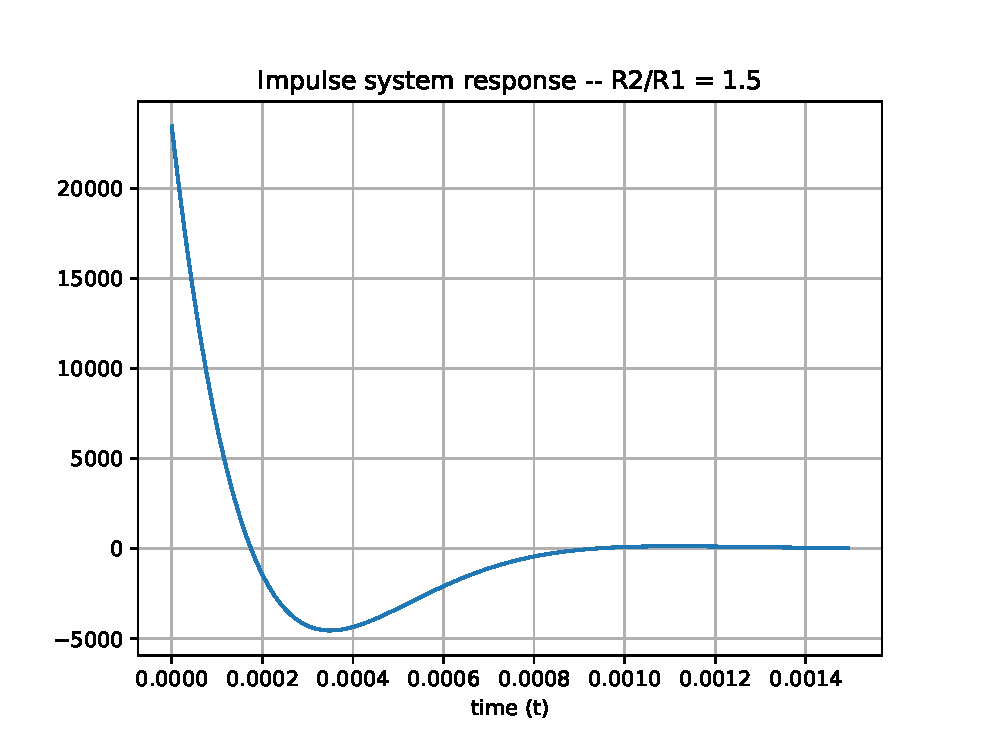
\includegraphics[width=\columnwidth]{./figs/ee18btech11044/ee18btech11044_3_14.eps}
\caption{}
\label{fig:ee18btech11044_3_14}
\end{figure}

\begin{figure}[!ht]
\centering
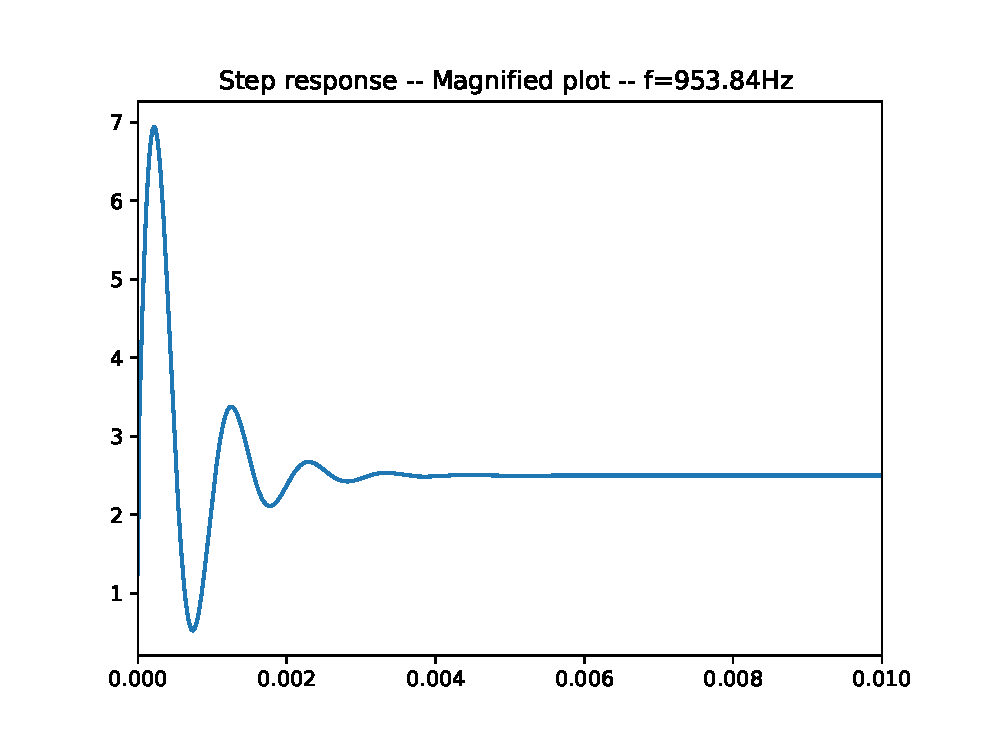
\includegraphics[width=\columnwidth]{./figs/ee18btech11044/ee18btech11044_3_15.eps}
\caption{}
\label{fig:ee18btech11044_3_15}
\end{figure}

%%%%%%%%%%%%%%%%%%%%%%%%%%%%%%spice simulation
\item Simulate the circuit shown in Fig \ref{fig:ee18btech11044_3_tikz_1} using spice simulators. Consider the ratio of $\frac{R_2}{R_1}$ = 1.5 and plot the output using a python script.

\solution

\begin{itemize}
\item Refer Fig \ref{fig:ee18btech11044_3_16} for the spice simulation output.  
\item You can find the netlist for the simulated circuit here:
\begin{lstlisting}
spice/ee18btech11044/ee18btech11044_3_4.net
\end{lstlisting}
\item You can find the python script used to generate the output here:
\begin{lstlisting}
spice/ee18btech11044/ee18btech11044_spice_3_7.py
\end{lstlisting}
\end{itemize}

\begin{figure}[!ht]
\centering
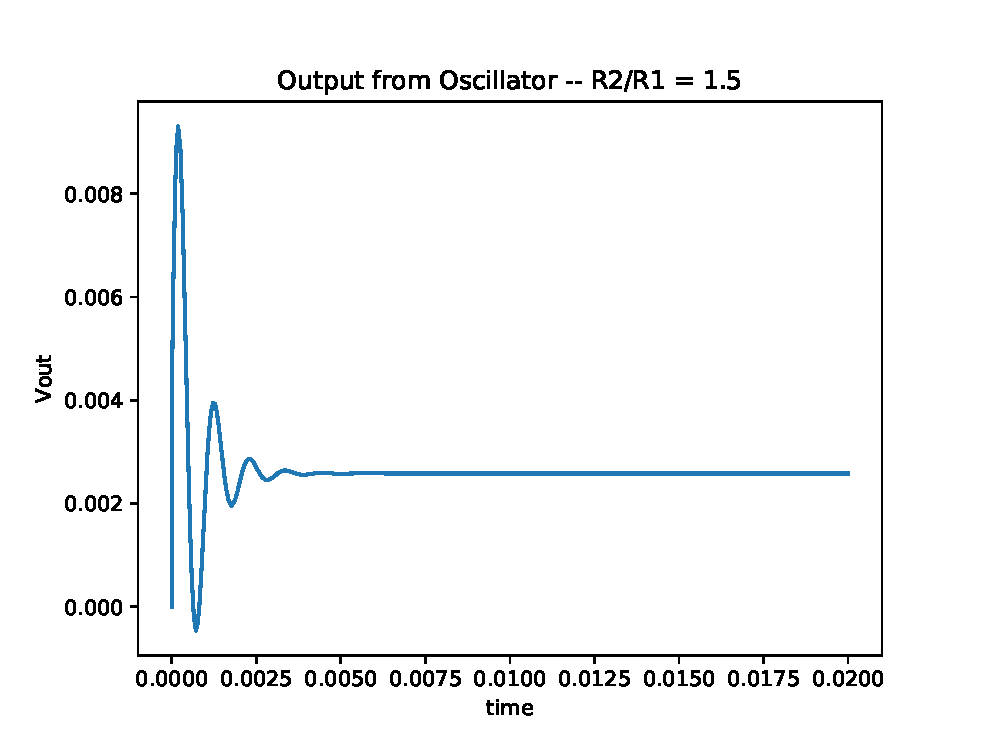
\includegraphics[width=\columnwidth]{./figs/ee18btech11044/ee18btech11044_3_16.eps}
\caption{}
\label{fig:ee18btech11044_3_16}
\end{figure}

%%%%%%%%%%%%%%%%%%%%%%%Frequency of spice simulation

\item Calculate the frequency of sinusoidal wave using plot generated from simulationfor the case where $\frac{R_2}{R_1} = 1.5$.
 
 \solution
 \begin{itemize}
     \item Consider a part of plot generated from simulation shown in the Fig \ref{fig:ee18btech11044_3_17}.
     \item Calculating the Time-period of the sinusoidal wave generated using the two points marked in the Fig \ref{fig:ee18btech11044_3_17}.
     \begin{align}
         T_0 = 0.00125 - 0.000191532 \\
         f_0 = 1/T_0 \\
         f_0 = 944Hz.
     \end{align}
     \item We get the frequencies calculated from the formulae and the plot to be very different.
     \item THe output predicted by python and spice simulation are matching in this case.
     \item Use this script to generate Fig \ref{fig:ee18btech11044_3_13}
\begin{lstlisting}
spice/ee18btech11044/ee18btech11044_spice_3_8.py
\end{lstlisting}
\item In this case because of the saturation voltage in op-amp we are getting a curve similar to square wave.
 \end{itemize}
 

 
\begin{figure}[!ht]
\centering
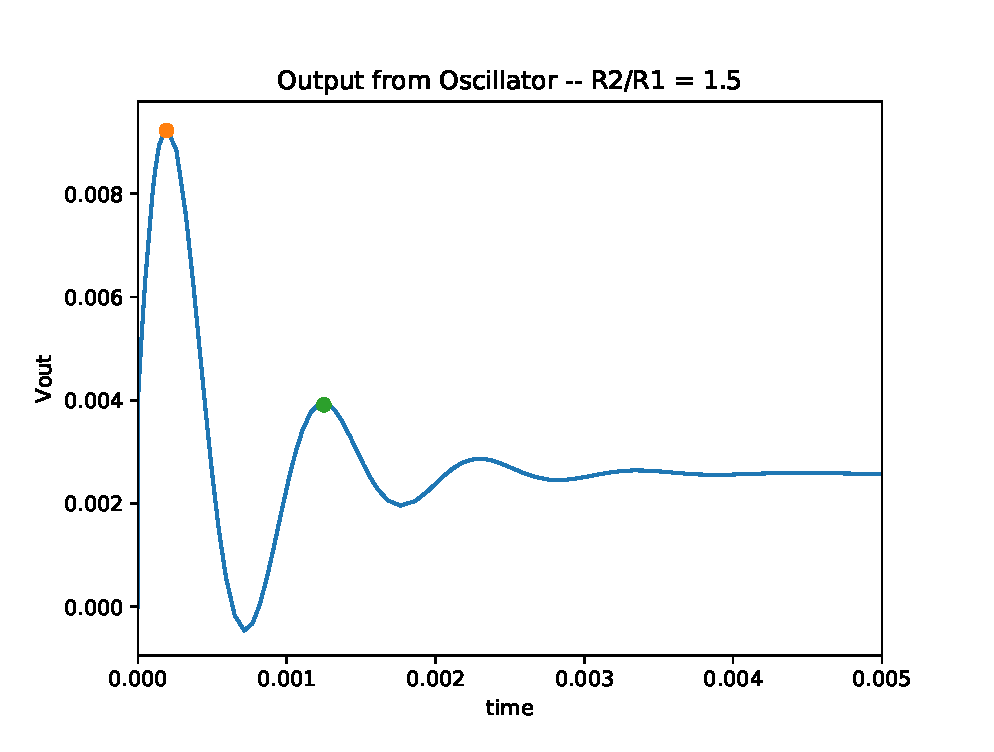
\includegraphics[width=\columnwidth]{./figs/ee18btech11044/ee18btech11044_3_17.eps}
\caption{}
\label{fig:ee18btech11044_3_17}
\end{figure}


\item Describe the output depending upon the nature of poles.

\solution 

\begin{itemize}
\item For purely imaginery poles, we expect a sinusoidal output (As in the case $\frac{R_2}{R_1}$ = 2).
\item For complex conjugate poles in right hand side of s-plane, we expect an exponentially increasing sinusoid as the output.(As in the case $2 < \frac{R_2}{R_1} < 4$).
\item For real and distinct poles in right hand side of s-plane, we expect an exponential  output.(As in the case $\frac{R_2}{R_1} > 4$).
\item For complex conjugate poles on the left hand side of splane, we expect an exponentially decreasing sinusoid.(As in the case $0 <  \frac{R_2}{R_1} < 2$.
\item It is not practical to simulate for real and distinct poles in left hand side of s plane as $R_2$ should be negative for that case. 
\item As you can observe behaviour of output generated by python scripts can be explained from the location of poles.
\item In the case of spice simulation, the output is always sinusoidal when $\frac{R_2}{R_1} > 2$ which is not the expected shape. 
\item For $\frac{R_2}{R_1} <= 2$ spice simulation is producing output of expected shape and frequency. 
\item Do not consider the frequency of impulse response from python plot in case-1 and case-4, as python is not able to calculate the Inverse laplace completely i have plotted using function signal.impulse(system) which generates a python plot of correct shape but frequency cannot be calculated from this plot.
\item Please find the code to calculate impulse response in Case-1.
\begin{lstlisting}
codes/ee18btech11044/ee18btech11044_3_13.py
\end{lstlisting}
\item \item Please find the code to calculate impulse response in Case-2.
\begin{lstlisting}
codes/ee18btech11044/ee18btech11044_3_14.py
\end{lstlisting}

\end{itemize}

\end{enumerate}

\end{document}
